\section{Resoconto delle attività di verifica}
	Questa sezione riporta un resoconto di tutte le metriche per le quali è stato possibile svolgere una misurazione allo stato attuale del progetto.

	\subsection{Qualità di Processo}
		\subsubsection{Processi Primari}		% 7 metriche - 7 impl
			\subsubsubsection{Analisi dei Requisiti}
				I valori registrati per ogni periodo relativi alle metriche per l'analisi dei requisiti sono i seguenti:
				\subsubsubsection*{Percentuale di requisiti obbligatori soddisfatti (PROS)}

\rowcolors{2}{lightRowColor}{darkRowColor}
\begin{longtable}{
	>{\centering}p{0.15\textwidth}
	>{\centering}p{0.15\textwidth}
	>{\centering}p{0.15\textwidth}
	>{\centering}p{0.15\textwidth}
	>{\centering\arraybackslash}p{0.15\textwidth} }

	\caption{Percentuale requisiti obbligatori soddisfatti (PROS)} \\

	\coloredTableHead
		\textbf{\color{white} Metrica} &
		\textbf{\color{white} RR} &
		\textbf{\color{white} RP} &
		\textbf{\color{white} RQ} &
		\textbf{\color{white}RA}
		\tabularnewline
	\endhead

	% contenuto tabella
	% esempio: Modulo & Min & Max \\
	PROS & 0\% & 42\% & 100\% & 100\% \\

\end{longtable}


\subsubsubsection*{Percentuale di requisiti desiderabili soddisfatti (PRDesS)}

\rowcolors{2}{lightRowColor}{darkRowColor}
\begin{longtable}{
		>{\centering}p{0.15\textwidth}
		>{\centering}p{0.15\textwidth}
		>{\centering}p{0.15\textwidth}
		>{\centering}p{0.15\textwidth}
		>{\centering\arraybackslash}p{0.15\textwidth} }
	
	\caption{Percentuale requisiti desiderabili soddisfatti (PRDesS)} \\
	
	\coloredTableHead
	\textbf{\color{white} Metrica} &
	\textbf{\color{white} RR} &
	\textbf{\color{white} RP} &
	\textbf{\color{white} RQ} &
	\textbf{\color{white}RA}
	\tabularnewline
	\endhead
	
	% contenuto tabella
	% esempio: Modulo & Min & Max \\
	PROS & 0\% & 0\% & 0\% & - \\
	
\end{longtable}


\subsubsubsection*{Percentuale di requisiti opzionali soddisfatti (PROpzS)}

\rowcolors{2}{lightRowColor}{darkRowColor}
\begin{longtable}{
		>{\centering}p{0.15\textwidth}
		>{\centering}p{0.15\textwidth}
		>{\centering}p{0.15\textwidth}
		>{\centering}p{0.15\textwidth}
		>{\centering\arraybackslash}p{0.15\textwidth} }
	
	\caption{Percentuale requisiti opzionali soddisfatti (PROpzS)} \\
	
	\coloredTableHead
	\textbf{\color{white} Metrica} &
	\textbf{\color{white} RR} &
	\textbf{\color{white} RP} &
	\textbf{\color{white} RQ} &
	\textbf{\color{white}RA}
	\tabularnewline
	\endhead
	
	% contenuto tabella
	% esempio: Modulo & Min & Max \\
	PROS & 0\% & 0\% & 0\% & - \\
	
\end{longtable}

			\pagebreak
			\subsubsubsection{Progettazione}
				I valori registrati per ogni periodo relativi alle metriche per la progettazione sono i seguenti:
	\subsubsubsection*{CBO}		%Grafico
	\subsubsubsection*{SFIN}
	\subsubsubsection*{SFOUT}
			\subsubsubsection{Codifica}
				I valori registrati per ogni periodo relativi alle metriche per la codifica sono i seguenti:

\subsubsubsection*{Complessità ciclomatica}
I valori sono riportati secondo lo schema \textit{valore minimo trovato - valore massimo trovato} per ogni modulo\ped{\textit{G}}.
\rowcolors{2}{lightRowColor}{darkRowColor}
\begin{longtable}{
		>{\centering}p{0.15\textwidth}
		>{\centering}p{0.15\textwidth}
		>{\centering}p{0.15\textwidth}
		>{\centering}p{0.15\textwidth}
		>{\centering\arraybackslash}p{0.15\textwidth} }

		\caption{Complessità ciclomatica} \\

	\coloredTableHead
	\textbf{\color{white} Modulo} &
	\textbf{\color{white} RR} &
	\textbf{\color{white} RP} &
	\textbf{\color{white} RQ} &
	\textbf{\color{white}RA}
	\tabularnewline
	\endhead

	% contenuto tabella
	% esempio: Modulo & Min & Max \\
	Etherless-cli & 0 & 3-13 & - & - \\
	Etherless-smart & 0 & 2 & 2-4 & - \\
	Etherless-server & 0 & 3-7 & - & - \\

\end{longtable}

\pagebreak
\subsubsubsection*{Rapporto linee di codice per linee di commento (RCC)}
I valori sono calcolati facendo la media della percentuale di commenti presente in ogni file appartenente al modulo\ped{\textit{G}}.
\rowcolors{2}{lightRowColor}{darkRowColor}
\begin{longtable}{
		>{\centering}p{0.15\textwidth}
		>{\centering}p{0.15\textwidth}
		>{\centering}p{0.15\textwidth}
		>{\centering}p{0.15\textwidth}
		>{\centering\arraybackslash}p{0.15\textwidth} }

		\caption{Rapporto linee di codice per linee di commento} \\

	\coloredTableHead
	\textbf{\color{white} Modulo} &
	\textbf{\color{white} RR} &
	\textbf{\color{white} RP} &
	\textbf{\color{white} RQ} &
	\textbf{\color{white}RA}
	\tabularnewline
	\endhead

	% contenuto tabella
	% esempio: Modulo & Min & Max \\
	Etherless-cli & 0 & 0.04 & - & - \\
	Etherless-smart & 0 & 0.13 & 0.11 & - \\
	Etherless-server & 0 & 0.06 & - & - \\

\end{longtable}

\subsubsubsection*{Numero di parametri per metodo}
I valori sono riportati secondo lo schema \textit{valore minimo trovato - valore massimo trovato} per ogni modulo\ped{\textit{G}}.
\rowcolors{2}{lightRowColor}{darkRowColor}
\begin{longtable}{
		>{\centering}p{0.15\textwidth}
		>{\centering}p{0.15\textwidth}
		>{\centering}p{0.15\textwidth}
		>{\centering}p{0.15\textwidth}
		>{\centering\arraybackslash}p{0.15\textwidth} }

		\caption{Numero di parametri per metodo} \\

	\coloredTableHead
	\textbf{\color{white} Modulo} &
	\textbf{\color{white} RR} &
	\textbf{\color{white} RP} &
	\textbf{\color{white} RQ} &
	\textbf{\color{white}RA}
	\tabularnewline
	\endhead

	% contenuto tabella
	% esempio: Modulo & Min & Max \\
	Etherless-cli & 0 & 0-1 & - & - \\
	Etherless-smart & 0 & 0-2 & 0-5 & - \\
	Etherless-server & 0 & 0-2 & - & - \\

\end{longtable}


\subsubsubsection*{Numero di attributi per classe}
I valori sono riportati secondo lo schema \textit{valore minimo trovato - valore massimo trovato} per ogni modulo\ped{\textit{G}}.
\rowcolors{2}{lightRowColor}{darkRowColor}
\begin{longtable}{
		>{\centering}p{0.15\textwidth}
		>{\centering}p{0.15\textwidth}
		>{\centering}p{0.15\textwidth}
		>{\centering}p{0.15\textwidth}
		>{\centering\arraybackslash}p{0.15\textwidth} }

		\caption{Numero di attributi per classe} \\

	\coloredTableHead
	\textbf{\color{white} Modulo} &
	\textbf{\color{white} RR} &
	\textbf{\color{white} RP} &
	\textbf{\color{white} RQ} &
	\textbf{\color{white}RA}
	\tabularnewline
	\endhead

	% contenuto tabella
	% esempio: Modulo & Min & Max \\
	Etherless-cli & 0 & 1-2 & - & - \\
	Etherless-smart & 0 & 5 & 1-7 & - \\
	Etherless-server & 0 & 0 & - & - \\

\end{longtable}

		
		\subsubsection{Processi di Supporto}	% 5 metriche - 3 impl
			\subsubsubsection{Documentazione}
				\subsection{Documentazione}
    \subsubsection{Descrizione}
      Questa sezione fornisce le norme per la stesura, la verifica e l'approvazione dei documenti. Tali regole vanno seguite in tutti i documenti ufficiali prodotti durante il ciclo di vita del software, garantendo così la coerenza e la validità degli stessi.
      
	\subsubsection{Attività}
	  \subsubsubsection{Implementazione del processo}
	  Per ogni documento che si intende sviluppare è necessario identificare:
	  \begin{itemize}
	  	\item \textbf{titolo o nome}: che sia significativo ed ufficiale;
	  	\item \textbf{scopo}: che espliciti il contenuto generale del documento e la sua funzionalità come documentazione di progetto;
	  	\item \textbf{destinatari}: che indichi i soggetti a cui il documento è destinato, o coloro i quali sono tenuti a prenderne visione;
	  	\item \textbf{procedure di gestione}: che guidino i responsabili nello sviluppo corretto e normato del documento, durante tutto il suo ciclo di vita;
	  	\item \textbf{versionamento}: pianificazione di versioni intermedie e finali del documento.
	  \end{itemize}
      
    \subsubsubsection*{Ciclo di vita dei documenti}
      Ogni documento attraversa diversi stadi:
      \begin{itemize}
        \item \textbf{Creazione e strutturazione del documento:} il documento viene creato nella sua directory di appartenenza (secondo le indicazioni presenti nella sezione "Documenti interni ed esterni"), e viene stesa la sua struttura generale. Viene utilizzato un template\ped{\textit{G}} \LaTeX{}\ped{\textit{G}} (descritto nella sezione \textsection3.1.2.2);
        
        \item \textbf{Stesura:} scrittura effettiva dei contenuti del documento da parte di un redattore\ped{\textit{G}}. Ogni contenuto scritto dal redattore\ped{\textit{G}} deve essere prontamente revisionato da un Verificatore per garantirne la validità;
       
        \item \textbf{Verifica:} attività eseguita dai Verificatori, i quali si occupano di controllare che il documento sia conforme alle 
        \textit{\NdP{} v3.0.0}, sia sintatticamente che semanticamente. Alla fine di ogni controllo, il resoconto della verifica viene consegnato al Responsabile di Progetto che provvede a notificare il redattore\ped{\textit{G}} in caso di errori, riportando il documento al passo di "Stesura". Quando la fase di verifica finale non rileva ulteriori errori, il Responsabile passa il documento al processo di "Approvazione";
        
        \item \textbf{Approvazione:} in questa fase i Verificatori hanno terminato i controlli finali con esito positivo, comunicandoli al Responsabile, il quale si occupa di approvare il documento e preparare il rilascio.
      \end{itemize}
  	\subsubsubsection*{Destinatari}
  	Ogni documento deve essere classificato come Interno o Esterno:
  	\begin{itemize}
  		\item \textbf{Interno:} il documento viene utilizzato all'interno del team;
  		\item \textbf{Esterno:} il documento viene condiviso con il Committente\ped{\textit{G}} ed il Proponente\ped{\textit{G}}.
  	\end{itemize}
	Di seguito sono elencati i documenti ufficiali prodotti e la loro classificazione in uso Interno o Esterno:
	\begin{itemize}
		\item \textbf{Norme di Progetto}:
		documento ad uso Interno.\\
		Lo scopo delle \textit{\NdP{}} è descritto nella sezione \textsection1.1 "Scopo del Documento", di questo stesso documento;
		
		\item \textbf{Studio di Fattibilità}:
		documento ad uso Interno.\\
		Lo \textit{\SdF{}} ha l'obiettivo di esporre (brevemente) ogni capitolato\ped{\emph{G}} e di elencare per ognuno gli aspetti positivi e le criticità che il team ha individuato;
		
		\item \textbf{Glossario}:
		documento ad uso Esterno.\\
		Il \Glossario{}  ha lo scopo di disambiguare alcuni termini che compaiono all'interno dei documenti e vengono utilizzati nelle comunicazioni interne;
		
		\item \textbf{Analisi dei Requisiti}:
		documento ad uso Esterno.\\
		Lo  scopo  dell'\textit{\AdR{}} è di esporre dettagliatamente i requisiti individuati per lo sviluppo del capitolato\ped{\emph{G}} scelto;
		
		\item \textbf{Piano di Progetto}:
		documento ad uso Esterno.\\
		Lo scopo del \textit{\PdP{}} è di organizzare le attività in modo da gestire le risorse disponibili in termini di tempo e "forza lavoro";
		
		\item \textbf{Piano di Qualifica}:
		documento ad uso Esterno.\\
		Lo scopo del \textit{\PdQ{}} è di presentare i metodi di verifica e validazione implementati dal gruppo, per garantire la qualità del prodotto\ped{\textit{G}} e dei processi adottati.
		
		\item \textbf{Develop Manual}:
		documento ad uso Esterno in lingua inglese.\\
		Lo scopo del \textit{Develop Manual} è di presentare il prodotto nei suoi dettagli implementativi. Si rivolge principalmente a sviluppatori che si occuperanno della manutenzione o di future estensioni del software.
		
		\item \textbf{User Manual}:
		documento ad uso Esterno i lingua inglese.\\
		Lo scopo del \textit{User Manual} è di presentare il prodotto ad un utilizzatore, trattando nello specifico funzionalità e benefici che porta l'utilizzo del software sviluppato.
		
	\end{itemize}

   	\subsubsubsection{Design e sviluppo}
      \subsubsubsection*{Template \LaTeX}
        Per uniformare la struttura dei documenti il gruppo ha deciso di creare un template\ped{\textit{G}} \LaTeX{}\ped{\textit{G}}, da utilizzare per la stesura di tutti i documenti ufficiali. Il template\ped{\textit{G}} è contenuto nella cartella \LaTeX{}\ped{\textit{G}}, la cui struttura è la seguente:
        \begin{itemize}
          \item \textbf{common\_commands.tex:} file che contiene la definizione di nuovi comandi \LaTeX{}\ped{\textit{G}} per l'inserimento nel flusso di testo di termini ricorrenti:
            \begin{itemize}
              \item \textbf{informazioni sul gruppo:} nome del gruppo e indirizzo email;
              \item \textbf{informazioni sul progetto:} nome del progetto e nomi del Proponente\ped{\textit{G}} e del Committente\ped{\textit{G}};
              \item \textbf{membri del gruppo:} nomi dei membri del gruppo \Gruppo;
              \item \textbf{nomi dei documenti:} nomi dei documenti ufficiali.
            \end{itemize}
          \item \textbf{configs.tex:} contiene i comandi per l'inclusione dei necessari pacchetti \LaTeX{}\ped{\textit{G}} e la definizione dell'aspetto grafico generale dei documenti;
          \item \textbf{en_configs.tex:} versione inglese del file 'configs.txt';
          \item \textbf{copertina.tex:} contiene il codice \LaTeX{}\ped{\textit{G}} per la copertina, ovvero la prima pagina di ogni documento (la cui struttura è descritta nella sezione \textsection3.1.2.2);
          \item \textbf{en_copertina.tex:}  versione inglese del file 'copertina.txt';
          \item \textbf{Template:} directory che contiene la struttura "classica" di un documento (quest'ultima viene descritta di seguito).
        \end{itemize}
        La directory Template ha la seguente struttura:
        \begin{itemize}
          \item \textbf{config:} directory che contiene un solo file: "commands.tex", all'interno del quale sono inseriti dei comandi specifici per il documento considerato (es. nome del documento, stato di approvazione, ecc...). I comandi devono essere adeguatamente modificati per ogni rispettivo documento;
          \item \textbf{res:} directory che contiene due cartelle:
            \begin{itemize}
              \item \textbf{img:} contiene le immagini utilizzate all'interno del documento;
              \item \textbf{sections:} contiene le varie sezioni del documento e un file "changelog.tex", ovvero il codice per il registro delle modifiche.
            \end{itemize}
          \item \textbf{document.tex:} il file contiene la struttura generica di un documento, includendo le sezioni necessarie contenute nella cartella res.
        \end{itemize}
        %da espandere

      \subsubsubsection*{Copertina}
        La copertina è la prima pagina di ogni documento e contiene alcune informazioni generali, in lingua Italiano o Inglese a seconda del documento trattato:
        \begin{itemize}
          \item Logo del gruppo \Gruppo{};
          \item Nome del gruppo e nome del capitolato\ped{\emph{G}} scelto: \Gruppo{} - \NomeProgetto{};
          \item Nome del documento (nel caso dei Verbali\ped{\textit{G}} accompagnato dalla data della riunione).
        \end{itemize}
        Queste informazioni sono seguite da una struttura tabellare, che contiene dettagli pertinenti al singolo documento:
        \begin{itemize}
          \item \textbf{Versione:} versione attuale del documento (vedi sezione \textsection3.2);%aggiungere sezione norme di Versionamento
          \item \textbf{Approvazione:} nome e cognome del Responsabile di progetto;
          \item \textbf{Redazione:} nome e cognome dei redattori\ped{\textit{G}} del documento;
          \item \textbf{Verifica:} nome e cognome dei Verificatori;
          \item \textbf{Stato:} stato del ciclo di vita in cui si trova il documento (vedi sezione \textsection3.1.2.1 paragrafo "Ciclo di vita dei documenti");
          \item \textbf{Uso:} indica se il documento è ad uso Interno o Esterno;
          \item \textbf{Destinato a:} elenco dei destinatari del documento (vedi sezione \textsection3.1.2.1 paragrafo del singolo documento);
    	\end{itemize}
    	Tale struttura è infine seguita da alcune informazioni aggiuntive, allineate al centro del documento:
    	\begin{itemize}
          \item \textbf{Descrizione:} breve descrizione del documento;
          \item \textbf{Email:} indirizzo email del gruppo \Gruppo{}.
   		\end{itemize}

      \subsubsubsection*{Registro delle modifiche}
        Inizia nella seconda pagina del documento e contiene un resoconto delle modifiche apportate al documento, strutturate in forma tabellare.\\
        Questa sezione è presente anche nei Verbali\ped{\textit{G}} di riunione, nei quali si limita alla stesura, la verifica e l'approvazione del documento in questo ordine, per evitare modifiche retroattive ai Verbali.\\
        Ogni riga rappresenta una modifica ed è suddivisa in cinque colonne:
        \begin{itemize}
          \item \textbf{V:} aggiornamento progressivo della versione;
          \item \textbf{Data:} data del rilascio della versione;
          \item \textbf{Nominativo:} nome e cognome del membro del gruppo che ha effettuato la modifica e corrispondente ruolo ricoperto;
          \item \textbf{Descrizione:} breve descrizione della modifica effettuata;
          \item \textbf{Verifica:} nome e cognome del verificatore che ha revisionato le modifiche apportate.
        \end{itemize}

      \subsubsubsection*{Indice}
        L'indice si trova nella pagina successiva e ha lo scopo di aiutare nella navigazione del documento e riassumerne la struttura in maniera visuale.\\
        Nell'indice sono elencati i numeri delle sezioni, seguiti dal titolo e dal numero di pagina. Ogni riga dell'indice è un link che porta alla sezione specificata del documento.\\
        L'indice dei contenuti puó essere seguito da un indice delle immagini e un indice delle tabelle.

      \subsubsubsection*{Contenuto}
        Tutte le pagine successive sono occupate dal contenuto e sono strutturate come segue:
        \begin{itemize}
          \item in alto a destra il nome del documento, corredato dalla sua versione;
          \item in alto a sinistra il logo del gruppo \Gruppo{};
          \item il contenuto della pagina diviso da intestazione e piè di pagina con una riga orizzontale;
          \item in basso a destra il numero di pagina nel formato:
          \begin{center}
            \textbf{Pagina [numero di pagina] di [numero totale di pagine]}.
          \end{center}
        \end{itemize}

      \subsubsubsection*{Verbali}
        Seguono la stessa struttura generale degli altri documenti, ma hanno un'organizzazione specifica del contenuto, in particolare sono suddivisi in:
        \begin{itemize}
          \item \textbf{Informazioni generali:} che contengono le informazioni dell'incontro e l'ordine del giorno.

             Le informazioni dell'incontro sono:
               \begin{itemize}
                 \item \textbf{Luogo:} il luogo dove si è svolta la riunione (in alternativa il mezzo utilizzato es. Skype\ped{\textit{G}});
                 \item \textbf{Data:} il giorno in cui si è svolta la riunione;
                 \item \textbf{Ora di inizio:} l'orario di inizio della riunione;
                 \item \textbf{Ora di fine:} l'orario di fine della riunione;
                 \item \textbf{Partecipanti:} elenco dei partecipanti alla riunione;
                 \item \textbf{Segretario:} redattore\ped{\textit{G}} del \Verbale{}\ped{\textit{G}}.
               \end{itemize}
			L'ordine del giorno contiene un elenco degli argomenti di discussione previsti per l'incontro.
          \item \textbf{\Verbale{}}\ped{\textit{G}}\textbf{:} che contiene la descrizione e un riassunto degli argomenti elencati nell'ordine del giorno, suddivisi in sezioni;
          \item \textbf{Riepilogo delle decisioni:} contiene il resoconto delle decisioni prese durante la riunione, in forma tabellare. Ogni decisione è identificata da un codice scritto in forma:
          \begin{center}
            \textbf{V[T]\_[numero dell'incontro].[numero progressivo]}
          \end{center}
          dove [T] indica il tipo di \Verbale{}\ped{\textit{G}} che puó essere Interno (I) o Esterno (E).
        \end{itemize}
	\subsubsubsection{Produzione}
		Per la scrittura e produzione di documentazione standardizzata, sono state introdotte le seguenti norme tipografiche.
      \subsubsubsection*{Nomi dei file}
        I nomi dei file seguono le seguenti regole:
        \begin{itemize}
          \item sono composti di diverse parole, con la prima lettera minuscola, fatta eccezione per i Verbali che, come descritto in seguito, iniziano per VI oppure VE;
          \item ogni parola è separata da un underscore;
          \item il nome del file corrisponde al nome del documento senza escludere le preposizioni, ad eccezione dei Verbali\ped{\textit{G}}, come già menzionato.
        \end{itemize}
        I Verbali seguono quindi delle regole differenti, a causa della loro unicità rispetto ad altri documenti. Sono nominati seguendo la struttura:
        \begin{center}
          \textbf{{V[T]\_[data]}}
        \end{center}
        \begin{itemize}
          \item \textbf{[T]:} indica il tipo di \Verbale{}\ped{\textit{G}} che puó essere Interno (I) o Esterno (E);
          \item \textbf{[data]:} indica la data della riunione in formato "YYYY\_MM\_DD", ovvero anno (YYYY), mese (MM) e giorno (DD), separati da underscore.
        \end{itemize}
        Esempi di nomi corretti:
        \begin{itemize}
          \item per un documento qualunque: nome\_di\_file.tex;
          \item per un \Verbale{}\ped{\textit{G}}: VI\_2020\_03\_16.tex.
        \end{itemize}
    	\noindent Inoltre, si è deciso di adottare delle convenzioni anche per la parola "verbale", in particolare:
    	\begin{itemize}
    		\item nel caso in cui essa compaia al singolare, deve essere riportata in corsivo e con la prima lettera maiuscola;
    		\item nel casi in cui essa compaia al plurale, deve essere riportata solamente con la prima lettera maiuscola.
    	\end{itemize}

      \subsubsubsection*{Stile del testo}
        Le seguenti norme vanno seguite per l'utilizzo di particolari stili di testo:
        \begin{itemize}
          \item \textbf{Grassetto:} usato se necessario all'inizio delle voci di un elenco puntato, a titoli o a termini significativi;
          \item \textbf{Corsivo:} usato per evidenziare proposizioni particolari all'interno del testo, in particolare il nome dei documenti ufficiali, il nome del Proponente\ped{\textit{G}}, il nome del progetto \textit{\NomeProgetto} e il nome del gruppo \textit{\Gruppo{}};
          \item \textbf{Maiuscoletto:} usato per la "G" a pedice che indica le parole presenti nel \Glossario{}.
        \end{itemize}
        Quando all'interno del testo vengono riferiti dei particolari documenti (es.: \AdR), vanno seguite le seguenti regole:
        \begin{itemize}
          \item indicare con lettera maiuscola le iniziali (es. \AdR), senza la versione del documento, il tutto in corsivo;
          \item se si fa riferimento al documento vero e proprio o a qualcosa in esso contenuto, va aggiunta la versione del documento nel formato:
          \begin{center}
              \textbf{v[X].[Y].[Z]}
          \end{center}
          (es. Riferendosi ad una sezione specifica "[\dots{}] come indicato nella \textsection5.1 dell'\AdR{} v1.1.0[\dots{}]").
        \end{itemize}
      \subsubsubsection*{Termini del Glossario}
      	Le norme relative ai termini da inserire nel \Glossario{} sono:
        \begin{itemize}
          \item ogni termine del \Glossario{} deve essere contrassegnato, in ogni sua istanza, da una G maiuscola a pedice;
          \item le istanze dei termini del \Glossario{} presenti nei titoli non necessitano della G maiuscola a pedice.
        \end{itemize}

      \subsubsubsection*{Elenchi puntati}
          Ogni voce di un elenco puntato deve aderire alle norme seguenti:
          \begin{itemize}
            \item deve iniziare con la lettera minuscola;
            \item deve essere seguita da un ";", fatta eccezione per l'ultimo elemento che deve essere seguito da un punto;
            \item puó iniziare con dei termini in grassetto e/o con prima lettera maiuscola nel caso in cui il resto della voce sia una descrizione di quei termini.
          \end{itemize}

      \subsubsubsection*{Date e orari}
        In conformità allo standard ISO 8601, le date devono essere scritte usando il formato:
        \begin{center}
          \textbf{YYYY-MM-DD}
        \end{center}
        ovvero anno in quattro cifre (YYYY), mese in due cifre (MM) e giorno in due cifre (DD).\\
        Gli orari devono essere scritti usando il formato:
        \begin{center}
          \textbf{HH.MM}
        \end{center}
        ovvero l'ora in due cifre (HH) e i minuti in due cifre (MM).

      \subsubsubsection*{Tabelle e immagini}
        Le tabelle sono sempre corredate da un titolo ed un'indicizzazione separata dal normale contenuto.\\
        Le immagini sono accompagnate da una didascalia ed un'indicizzazione, anch'essa separata dal normale contenuto.

      \subsubsubsection*{Sigle e abbreviazioni}
        Nella stesura dei documenti possono venire menzionate diverse sigle:
        \begin{itemize}
          \item sigle per i ruoli di progetto:
            \begin{itemize}
              \item \textbf{Rp:} Responsabile di Progetto;
              \item \textbf{As:} Amministratore;
              \item \textbf{An:} Analista;
              \item \textbf{Pt:} Progettista;
              \item \textbf{Pr:} Programmatore;
              \item \textbf{Vf:} Verificatore.
            \end{itemize}
          \item sigle per i nomi dei documenti:
            \begin{itemize}
              \item \textbf{SdF:} Studio di Fattibilità;
              \item \textbf{PdQ:} Piano di Qualifica;
              \item \textbf{PdP:} Piano di Progetto;
              \item \textbf{NdP:} Norme di Progetto;
              \item \textbf{AdR:} Analisi dei Requisiti;
              \item \textbf{G:} Glossario.
            \end{itemize}
          \item sigle per revisioni del progetto:
            \begin{itemize}
              \item \textbf{RR:} Revisione dei Requisiti;
              \item \textbf{RP:} Revisione di Progettazione;
              \item \textbf{RQ:} Revisione di Qualifica;
              \item \textbf{RA:} Revisione di Accettazione.
            \end{itemize}
        \end{itemize}
	\subsubsubsection{Manutenzione}
		Qualora sia necessario apportare modifiche o aggiornamenti ad un documento, si fa riferimento alle norme specificate nelle sezioni \textsection{3.2} e \textsection{3.3} di questo stesso documento.
	\subsubsection{Metriche}
		\subsubsubsection{Indice di Gulpease}
			\begin{itemize}
				\item{\textbf{Descrizione}}: è un indice di leggibilità di un testo tarato sulla lingua italiana. Considera due variabili linguistiche: la lunghezza della parola e la lunghezza della frase rispetto al numero di lettere;
				\item{\textbf{unità di misura}}: la metrica è espressa tramite un numero intero;
				\item{\textbf{formula}}: $ IG=89+\frac{300 \times \#frasi -10\times \#lettere}{\#parole} $;
				\item{\textbf{risultato}}: il risultato è compreso tra 0 e 100, dove il valore 100 indica il grado più alto di leggibilità e 0 il più basso. In particolare:
					\begin{itemize}
						\item se il risultato è inferiore a 80, il testo è considerato di difficile lettura per chi ha la licenza elementare;
						\item se il risultato è inferiore a 60, il documento è considerato di difficile lettura per chi ha la licenza media;
						\item se il risultato è minore di 40, il documento è considerato di difficile lettura per chi ha un diploma superiore.
					\end{itemize}
			\end{itemize}

		\subsubsubsection{Formula di Flesch}
		\begin{itemize}
			\item{\textbf{Descrizione}}: formula utilizzata per misurare la leggibilità di un testo inglese;
			\item{\textbf{unità di misura}}: la metrica è espressa tramite un numero decimale;
			\item{\textbf{formula}}: $ F = 206,835 - (84,6 \times S) - (1,015 \times P) $, dove:
				\begin{itemize}
					\item S indica il numero medio di sillabe per parola;
					\item P indica il numero medio di parole per frase.
				\end{itemize}
			\item{\textbf{risultato}}: il risultato è compreso tra 0.0 e 100.0, in particolare:
				\begin{itemize}
					\item se il risultato è compreso tra 0.0 e 30.0 il documento è considerato molto difficile da leggere, adatto a lettori laureati;
					\item se il risultato è compreso tra 30.0 e 50.0 il documento è leggibile per studenti universitari;
					\item se il risultato è compreso tra 50.0 e 70.0 il documento è leggibile per chi possiede un diploma superiore;
					\item se il risultato è compreso tra 70.0 e 90.0 il documento è leggibile per chi possiede una licenza media;
					\item se il risultato è compreso tra 90.0 e 100.0 il documento viene considerato di facile lettura per un qualsiasi lettore.
				\end{itemize}
		\end{itemize}

		\subsubsubsection{Correttezza ortografica}
		\begin{itemize}
			\item{\textbf{Descrizione}}: permette di misurare la correttezza a livello lessicografico del documento;
			\item{\textbf{unità di misura}}: la metrica è espressa tramite un numero intero;
			\item{\textbf{formula}}: il valore coincide con il numero di errori ortografici presenti, cioè: $ CO = \#numero\_errori\_ortografici $;
			\item{\textbf{risultato}}:
				\begin{itemize}
					\item se il risultato è pari a 0, il documento è considerato corretto e non presenta errori ortografici;
					\item se il risultato è maggiore di 0, allora il documento presenta almeno un errore ortografico.
				\end{itemize}
		\end{itemize}

    \subsubsection{Strumenti}
      \subsubsubsection{\LaTeX}
        Per la stesura della documentazione si è scelto il linguaggio di markup \LaTeX{}\ped{\textit{G}}. Nonostante non sia di immediata comprensione, quest'ultimo permette di scrivere documenti in modo collaborativo, modulare e scalabile.

      \subsubsubsection{File condivisi di Microsoft Teams}
        Si utilizza la condivisione di file interna a Microsoft Teams\ped{\textit{G}} per file utili non ufficiali. Questa piattaforma offre infatti funzionalità per il lavoro simultaneo sugli stessi file, che risulta utile per l'organizzazione interna del lavoro di gruppo.

      \subsubsubsection{Editor di testo}
        Si è demandata la scelta dell'editor di testo ai singoli membri del gruppo per permettere un lavoro più efficiente, data la familiarità di ognuno con diversi editor e ambienti di lavoro.

	  \subsubsubsection{Microsoft Excel}
		Software per la creazione e la gestione di fogli elettronici, distribuito da Microsoft come parte della suite Microsoft Office. Utilizzato per funzioni di calcolo, produzione di tabelle, grafica e diagrammi. \\
		\begin{figure}[h!]
			\centering
			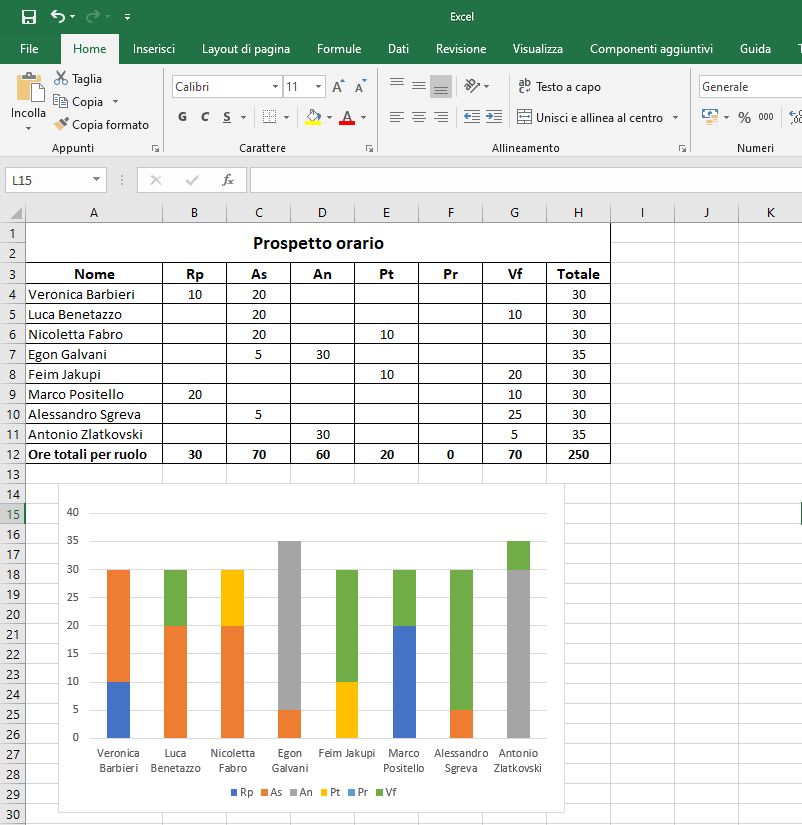
\includegraphics[scale=0.62]{./res/img/excel.png}
			\caption{Microsoft Excel\ped{\textit{G}}}
		\end{figure}
		\pagebreak
	  \subsubsubsection{GanttProject}
	    Software per la gestione dei progetti basato su Java\ped{\textit{G}}. Utilizzato principalmente per la creazione di diagrammi di Gantt, ovvero strumenti in grado di rappresentare le tempistiche e le attività di un progetto, per tracciare quindi il suo avanzamento.
	    \begin{figure}[h!]
	    	\centering
	    	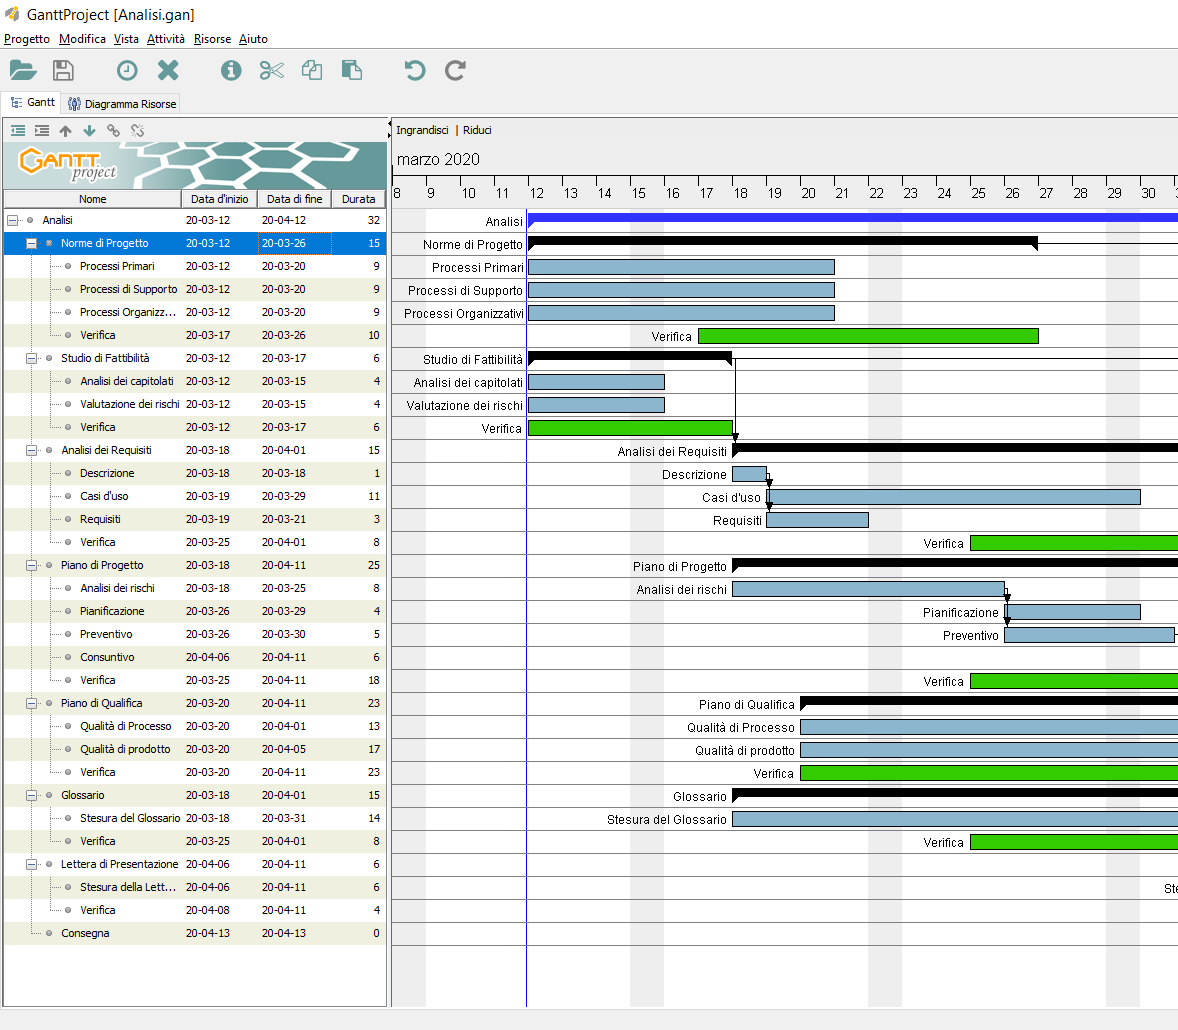
\includegraphics[scale=0.5]{./res/img/diagr_gantt.png}
	    	\caption{GanttProject\ped{\textit{G}}}
	    \end{figure}
	    \pagebreak

			\subsubsubsection{Gestione della Qualità}
				\paragraph{Percentuale di metriche soddisfatte (PMS)}
	Nel seguente grafico vengono riportati i valori PMS, calcolati in differenti momenti di maturazione del progetto.\\
	Nella prima fase del progetto si può osservare che il numero di metriche soddisfatte può essere inferiore al valore minimo accettabile, in quanto nel calcolo sono incluse le metriche da calcolare in futuro.
	\begin{center}
		\begin{tikzpicture} [scale = 0.9]
		\begin{axis}[
		xlabel={\textbf{Tempo}},
		ylabel={\textbf{Percentuale di metriche soddisfatte}},
		date coordinates in=x,
		ymin=0,
		ymax=100,
		xtick=data,
		xticklabel style={
			rotate=90,
			anchor=near xticklabel,
		},
		xticklabel=\year-\month-\day,
		]
		\addplot table [col sep=comma,x=date,y=value,blue] {res/sections/B/gestione_qualita/PMS.csv};
		\draw [line width=0.1, red](2020-3-05, 60)--(2020-5-20, 60);
		\legend{$PMS$};
		\end{axis}
		\end{tikzpicture} \\
	\end{center}
			\subsubsubsection{Verifica}
				\subsubsubsection*{Code Coverage}	

	\begin{figure}[H]
		\centering
		\begin{tikzpicture} [scale = 0.7]
		\begin{axis}[
		xlabel={\textbf{Tempo}},
		ylabel={\textbf{Code Coverage}},
		date coordinates in=x,
		ymin=78,
		ymax=100,
		xtick=data,
		xticklabel style={
			rotate=90,
			anchor=near xticklabel,
		},
		xticklabel=\year-\month-\day,
		]
	%	\addplot table [col sep=comma,x=date,y=value,blue] {res/sections/B/code_coverage/cli.csv};
	%	\addplot table [col sep=comma,x=date,y=value,blue] {res/sections/B/code_coverage/smart.csv};
		\addplot table [col sep=comma,x=date,y=value,blue] {res/sections/B/code_coverage/server.csv};
	
		\draw [line width=0.1, red](2020-6-1, 80)--(2020-6-30, 80);
		\legend{$Cli$ ,$Smart$ ,$Server$};
		\end{axis}
		\end{tikzpicture} 
		\caption{Code Coverage}
	\end{figure}

		
		\pagebreak		
		\subsubsection{Processi Organizzativi}	% 1 metrica - 1 impl
			\subsubsubsection{Gestione Organizzativa}
				\subsection{Gestione Organizzativa}

		\subsubsection{Descrizione}
			La gestione organizzativa è il processo che descrive le scelte sottostanti la suddivisione e il coordinamento del lavoro all'interno del progetto. Lo scopo principale di questo processo è fornire ai membri del gruppo un \PdP{} per l'organizzazione del lavoro, con focus sull'efficacia e l'efficienza. Nello specifico, le attività che costituiscono questo processo sono:
			\begin{itemize}
				\item {inizializzazione e definizione degli obiettivi;}
				\item {pianificazione e gestione di scadenze, rischi e risorse;}
				\item {esecuzione e controllo dei processi;}
				\item {revisione e valutazione;}
				\item {Definition of Done\ped{\textit{G}}.}
			\end{itemize}
			Le operazioni svolte durante queste attività vengono in seguito descritte indirettamente, attraverso l'esplicitazione delle mansioni dei vari ruoli di progetto.
			\subsubsection{Attività}
			\subsubsubsection{Gestione ruoli di progetto}
			Ciascun componente del gruppo ricopre un ruolo di progetto a rotazione, facendo sì che ogni membro possa assumere almeno una volta ciascuno di essi nel corso del progetto. Nel documento \PdP{} \textit{3.0.0} vengono organizzate e pianificate le attività assegnate ai specifici ruoli previsti nell'attività di progetto. Ciascun ruolo viene descritto di seguito.

			\subsubsubsection*{Responsabile di Progetto}
			Il Responsabile di Progetto è una figura essenziale, che partecipa al progetto dall'inizio fino alla fine. È responsabile delle decisioni e scelte che vengono intraprese, coordinando l'intero progetto. Rappresenta il gruppo di fronte a soggetti esterni, come Committente\ped{\textit{G}} e Proponente\ped{\textit{G}}.
			Riassunto delle mansioni:
			\begin{itemize}
				\item coordina, pianifica e controlla le attività;
				\item gestisce le risorse umane;
				\item approva la documentazione;
				\item approva l'offerta economica;
				\item preventiva l'analisi dei rischi e la loro eventuale gestione;
				\item determina e verifica le condizioni di completezza.
			\end{itemize}

			\subsubsubsection*{Amministratore}
			L'Amministratore è la figura che ha come compito principale il controllo e l'amministrazione dell'ecosistema lavorativo. Inoltre ha diretta responsabilità sull'efficienza e sulla capacità operativa dell'ambiente di lavoro.
			Riassunto delle mansioni:
			\begin{itemize}
				\item studia e ricerca strumenti che riducano il più possibile l'impiego di risorse umane e che automatizzino tutto ciò che è possibile fare attraverso l'utilizzo di software;
				\item ricerca soluzioni ai problemi legati alla difficoltà di gestione dei processi e risorse, attraverso la realizzazione o la ricerca di strumenti adatti a tale scopo;
				\item controlla le versioni e le configurazioni del prodotto\ped{\textit{G}};
				\item gestisce il versionamento della documentazione del progetto e della sua archiviazione;
				\item fornisce procedure e strumenti di monitoraggio/segnalazione, in modo da garantire un corretto controllo di qualità.
			\end{itemize}

			\subsubsubsection*{Analista}
			L'Analista è il responsabile delle attività di analisi. Deve effettuare studi e ricerche in maniera molto approfondita per conoscere bene il dominio\ped{\textit{G}} del problema. Non è necessario che partecipi al progetto fino al termine, ma il suo operato è fondamentale fin dalla fase iniziale, in quanto le sue scelte decisionali hanno un grande impatto sul successo dell'intero progetto.
			Riassunto delle mansioni:
			\begin{itemize}
				\item studia e definisce il problema da risolvere, rilevandone la complessità;
				\item compie l'analisi del dominio\ped{\textit{G}} delle richieste tramite lo studio dei bisogni, espliciti ed impliciti;
				\item compie l'analisi del dominio\ped{\textit{G}} applicativo determinando gli utilizzatori e l'ambiente di utilizzo;
				\item redige i documenti \AdR{} e \SdF{}.
			\end{itemize}

			\subsubsubsection*{Progettista}
			Il Progettista è la figura che si occupa delle scelte architetturali del progetto e ne influenza gli aspetti tecnici e tecnologici. Utilizzando le attività svolte dall'Analista, il Progettista ha il compito di trovare una soluzione attuabile, comprensibile e motivata.
			Riassunto delle mansioni:
			\begin{itemize}
				\item produce una soluzione attuabile, comprensibile e motivata;
				\item effettua scelte su aspetti progettuali, applicando al prodotto\ped{\textit{G}} soluzioni note ed ottimizzate;
				\item effettua scelte che portino ad avere un prodotto\ped{\textit{G}} facilmente manutenibile.
			\end{itemize}

			\subsubsubsection*{Programmatore}
			Il Programmatore è la figura responsabile della codifica del codice e della creazione delle componenti di supporto, indispensabili per poter effettuare le prove di verifica e di validazione.
			Riassunto delle mansioni:
			\begin{itemize}
				\item implementa in maniera precisa e scrupolosa le soluzioni generate dal Progettista;
				\item scrive codice sorgente altamente e facilmente manutenibile;
				\item si occupa del versionamento e della documentazione del codice prodotto\ped{\textit{G}};
				\item realizza strumenti per la verifica e la validazione del software.
			\end{itemize}

			\subsubsubsection*{Verificatore}
			Il Verificatore è la figura che ha il compito di effettuare una attenta verifica del prodotto\ped{\textit{G}}, dando particolare attenzione al rispetto delle normative di progetto. Oltre ad una grande conoscenza di tali norme, il verificatore deve avere buone capacità di giudizio.
			Riassunto delle mansioni:
			\begin{itemize}
				\item controlla che le attività svolte siano conformi alle normative stabilite;
				\item vigila sull'integrità del prodotto\ped{\textit{G}} ad ogni stadio del suo ciclo di vita.
				\item comunica eventuali errori identificati al responsabile dell'oggetto preso in esame.
			\end{itemize}

			\subsubsubsection{Gestione delle comunicazioni}
			\subsubsubsection*{Comunicazioni interne}
			Le comunicazioni interne sono gestite principalmente attraverso tre canali:
			\begin{itemize}
				\item \textbf{gruppo Telegram}\ped{\textit{G}}: dove è possibile scambiare rapidamente comunicazioni brevi ed informali, coinvolgendo l'intero team.
				\item \textbf{Microsoft Teams}\ped{\textit{G}}: piattaforma dotata di funzioni di messaggistica istantanea, con possibilità di creare canali specifici divisi per argomento, e videochiamata. Viene utilizzata per lo scambio di comunicazioni più consistenti e tecniche, come aggiornamenti sulle attività di Verifica o discussioni legate a specifiche attività.
				\item \textbf{GitHub}\ped{\textit{G}}: anche se meno focalizzato sulla comunicazione, il sistema di gestione Issue\ped{\textit{G}} di GitHub\ped{\textit{G}} consente di aggiornare rapidamente l'intero gruppo sull'avanzamento dei lavori.
			\end{itemize}
			\subsubsubsection*{Comunicazioni esterne}
			Le comunicazioni esterne, gestite principalmente dal Responsabile di progetto, avvengono attraverso due canali:
			\begin{itemize}
				\item \textbf{Gmail}\ped{\textit{G}}: per comunicare con il Committente\ped{\textit{G}} e, almeno inizialmente, con il Proponente\ped{\textit{G}} viene utilizzata la casella di posta elettronica creata appositamente per il team \Gruppo{}.
				\item \textbf{canale Slack}\ped{\textit{G}}: è stato concordato con il Proponente\ped{\textit{G}} \Proponente{} l'utilizzo della piattaforma Slack\ped{\textit{G}}, con un canale dedicato al gruppo \Gruppo{}. Viene utilizzata per rapidi scambi di informazioni o la pianificazione di eventuali incontri.
			\end{itemize}
			\subsubsubsection{Gestione delle riunioni}
			Le riunioni sono indette dal Responsabile di Progetto, il quale ha il compito di:
			\begin{itemize}
				\item definire la data e l'orario delle riunioni, sia interne che esterne, considerando la disponibilità dei partecipanti;
				\item stabilire l'oggetto della riunione;
				\item valutare le richieste relative alle riunioni da parte dei componenti del Team \Gruppo{} e dai soggetti esterni;
				\item verificare ed approvare il verbale\ped{\textit{G}} redatto dal Segretario della riunione, il quale verrà nominato ad inizio incontro;
			\end{itemize}
			I partecipanti devono presentarsi puntuali alle riunioni e, in caso di imprevisti, comunicarli con congruo preavviso.
			Le decisioni da intraprendere durante le riunioni, sono ritenute approvate nel caso di maggioranza da parte dei partecipanti.\\
			Al termine di ciascuna riunione viene redatto un \Verbale{}\ped{\textit{G}} da parte del Segretario, che deve contenere tutte le informazioni sulla riunione.
			\subsubsubsection*{Riunioni interne}
				Le riunioni interne sono aperte esclusivamente agli 8 membri del gruppo \Gruppo{}. Le occasioni di incontro sono ritenute valide esclusivamente in due modalità:
				\begin{itemize}
					\item \textbf{incontri in video-conferenza:} Effettuati tramite l'applicativo Microsoft Teams\ped{\textit{G}};
					\item \textbf{incontri di persona:} Effettuati trovandosi fisicamente in uno stesso luogo.
				\end{itemize}
				Considerata la situazione extra-progettuale relativa all'emergenza COVID-19\ped{\textit{G}}, le riunioni iniziali saranno effettuate esclusivamente a distanza tramite video-conferenza.
				Affinché le riunioni siano ritenute valide, all'incontro dovranno essere presenti almeno 6 componenti del team.

			\subsubsubsection*{Riunioni esterne}
				Le riunioni esterne comprendono tutti gli incontri che coinvolgono, oltre ai membri del team \Gruppo{}, anche altri soggetti esterni.\\
				Questi incontri sono tenuti telematicamente, fino al termine dell'emergenza COVID-19\ped{\textit{G}} e, successivamente, potranno tenersi attraverso riunioni fisiche. In caso di video-conferenza è da privilegiare lo strumento di comunicazione proposto dai soggetti esterni, similmente per le riunioni fisiche, in luoghi proposti dai soggetti esterni.\\
				Nel caso si scelga di usufruire dei locali di Torre Archimede è necessario chiedere il permesso al \TV{} all'indirizzo mail \href{mailto:tullio.vardanega@math.unipd.it}{tullio.vardanega@math.unipd.it}.
			\subsubsubsection{Gestione degli strumenti di coordinamento e versionamento}
			\subsubsubsection*{Issue Tracking System}
			Come già menzionato, il gruppo ha deciso di utilizzare come strumento per l'organizzazione del carico di lavoro, la componente Issue\ped{\textit{G}} Tracking System (ITS) della piattaforma GitHub\ped{\textit{G}}. Grazie a tale strumento, è possibile rappresentare ogni singolo compito tramite Issue\ped{\textit{G}}, che verranno assegnate ai rispettivi responsabili per essere svolte entro scadenze prestabilite. È possibile inoltre avere una visione d'insieme delle Issue\ped{\textit{G}} (aperte o chiuse), così che il Responsabile di Progetto o eventuali Amministratori possano facilmente gestire e monitorare l'andamento del progetto.
			La procedura seguita per l'assegnazione di una Issue\ped{\textit{G}} è la seguente:
			\begin{itemize}
				\item vengono decisi uno o più responsabili per la nuova Issue\ped{\textit{G}};
				\item viene inserito un titolo alla Issue\ped{\textit{G}}, che renda chiaro il suo obiettivo;
				\item viene impostata una scadenza per la Issue\ped{\textit{G}}, se precedentemente concordata;
				\item la Issue\ped{\textit{G}} viene concretamente assegnata ai responsabili scelti;
				\item viene associata un'etichetta alla Issue\ped{\textit{G}}, utile ad identificare il contesto in cui questa opera o a classificarne la tipologia;
				\item qualora il titolo non sia sufficientemente esplicativo, o sia necessario aggiungere ulteriori informazioni, viene aggiunto un breve riassunto dell'obiettivo della Issue\ped{\textit{G}};
			\end{itemize}
			Il processo viene completato con una conferma, che provoca un'immediata notifica a tutti i componenti del gruppo.

			\subsubsubsection*{Repository}
			Per la gestione del versionamento e l'archiviazione dei file di progetto, viene sfruttata la componente VCS\ped{\textit{G}} della piattaforma GitHub\ped{\textit{G}}. Gli Amministratori si sono occupati della creazione della repository\ped{\textit{G}} \textbf{etherless}, e dei Git\ped{\textit{G}} submodule (repository\ped{\textit{G}} annidate): \textbf{Documentazione}, \textbf{etherless-cli}, \textbf{etherless-smart}, \textbf{etherless-server},  ed è loro compito garantire l'ordine e la pulizia di quest'ultimi. Il contenuto dei repository\ped{\textit{G}} relativi alle componenti software è quindi soggetto a repentini cambiamenti, con però una più stabile struttura di base.\\
			La struttura del repository\ped{\textit{G}} \textbf{etherless}, è la seguente:
			\begin{itemize}
				\item \textbf{Submodule Documentazione}: riferimento all'ultimo commit\ped{\textit{G}} stabile della repository\ped{\textit{G}} \textit{Documentazione};
				\item \textbf{Submodule etherless-cli}: riferimento all'ultimo commit\ped{\textit{G}} stabile della repository\ped{\textit{G}} \textit{etherless-cli};
				\item \textbf{Submodule etherless-smart}: riferimento all'ultimo commit\ped{\textit{G}} stabile della repository\ped{\textit{G}} \textit{etherless-smart};
				\item \textbf{Submodule etherless-server}: riferimento all'ultimo commit\ped{\textit{G}} stabile della repository\ped{\textit{G}} \textit{etherless-server};
				\item \textbf{File .gitmodules}: file utilizzato per la configurazione dei Git\ped{\textit{G}} modules;
				\item \textbf{File README.md}: file descrittivo della repository\ped{\textit{G}} di progetto, contenente istruzioni per la sua esecuzione. Scritto in lingua inglese;
				\item \textbf{File package.json}: file utilizzato per effettuare l'installazione dei moduli\ped{\textit{G}} necessari all'esecuzione del prodotto\ped{\textit{G}};
				\item \textbf{File tsconfig.json}: file utilizzato per la configurazione di Typescript\ped{\textit{G}}.
			\end{itemize}
			La struttura della repository\ped{\textit{G}} \textbf{Documentazione}, è la seguente:
			\begin{itemize}
				\item \textbf{Cartella Esterni}: contiene i file e sotto-cartelle relativi ai documenti esterni del progetto;
				\item \textbf{Cartella Interni}: contiene i file e sotto-cartelle relativi ai documenti interni del progetto;
				\item \textbf{Cartella Latex}\ped{\textit{G}}: contiene i file template\ped{\textit{G}} e configurazioni per il layout dei documenti \LaTeX{}\ped{\textit{G}};
				\item \textbf{File .gitignore}: specifica i tipi di file che devono essere ignorati e non presenti all'interno della repository\ped{\textit{G}}. In particolare si desidera conservare solo file di tipo .tex, .pdf, .jpg e .png.
			\end{itemize}
			La struttura della repository\ped{\textit{G}} \textbf{etherless-cli}, è la seguente:
			\begin{itemize}
				\item \textbf{Cartella contracts}: contiene i file relativi agli smart contract\ped{\textit{G}};
				\item \textbf{Cartella src}: contiene i file e sotto-cartelle relativi al codice eseguibile del modulo\ped{\textit{G}} Etherless-cli;
				\item \textbf{File .editorconfig}: file di supporto agli sviluppatori, per mantenere uno stile di codifica consistente tra editor e IDE\ped{\textit{G}} diversi;
				\item \textbf{File .eslintrc.js}: file utilizzato per la configurazione di ESLint\ped{\textit{G}};
				\item \textbf{File .gitignore}: specifica i tipi di file che devono essere ignorati e non presenti all'interno della repository\ped{\textit{G}};
				\item \textbf{File README.md}: file descrittivo della repository\ped{\textit{G}} del modulo, contenente istruzioni per la sua esecuzione. Scritto in lingua inglese;
				\item \textbf{File package.json}: file utilizzato per effettuare l'installazione dei moduli\ped{\textit{G}} necessari all'esecuzione del prodotto\ped{\textit{G}};
				\item \textbf{File package-lock.json}: file utilizzato per l'installazione dei moduli\ped{\textit{G}} necessari all'esecuzione del prodotto\ped{\textit{G}};
				\item \textbf{File tsconfig.json}: file utilizzato per la configurazione di Typescript\ped{\textit{G}}.
			\end{itemize}
			La struttura della repository\ped{\textit{G}} \textbf{etherless-smart}, è la seguente:
			\begin{itemize}
				\item \textbf{Cartella contracts}: contiene i file relativi agli smart contract\ped{\textit{G}};
				\item \textbf{Cartella migrazioni}: contiene i file relativi alle migrazioni;
				\item \textbf{File .gitignore}: specifica i tipi di file che devono essere ignorati e non presenti all'interno della repository\ped{\textit{G}};
				\item \textbf{File README.md}: file descrittivo della repository\ped{\textit{G}} del modulo, contenente istruzioni per la sua esecuzione. Scritto in lingua inglese;
				\item \textbf{File package.json}: file utilizzato per effettuare l'installazione dei moduli\ped{\textit{G}} necessari all'esecuzione del prodotto\ped{\textit{G}};
				\item \textbf{File package-lock.json}: file utilizzato per l'installazione dei moduli\ped{\textit{G}} necessari all'esecuzione del prodotto\ped{\textit{G}};
				\item \textbf{File truffle-config.json}: file utilizzato per la configurazione di Truffle\ped{\textit{G}}.
			\end{itemize}
			La struttura della repository\ped{\textit{G}} \textbf{etherless-server}, è la seguente:
			\begin{itemize}
				\item \textbf{Cartella configs}: contiene i file relativi alle configurazioni generali;
				\item \textbf{Cartella contracts}: contiene i file relativi agli smart contract\ped{\textit{G}};
				\item \textbf{Cartella serverless}: contiene i file e sotto-cartelle relativi al framework\ped{\textit{G}} Serverless\ped{\textit{G}};
				\item \textbf{Cartella src}: contiene i file e sotto-cartelle relativi al codice eseguibile del modulo\ped{\textit{G}} Etherless-server;
				\item \textbf{Cartella test}: contiene i file e sotto-cartelle relativi ai test;
				\item \textbf{File .eslintrc.js}: file utilizzato per la configurazione di ESLint\ped{\textit{G}}.
				\item \textbf{File .gitignore}: specifica i tipi di file che devono essere ignorati e non presenti all'interno della repository\ped{\textit{G}};
				\item \textbf{File README.md}: file descrittivo della repository\ped{\textit{G}} del modulo, contenente istruzioni per la sua esecuzione. Scritto in lingua inglese;
				\item \textbf{File package.json}: file utilizzato per effettuare l'installazione dei moduli\ped{\textit{G}} necessari all'esecuzione del prodotto\ped{\textit{G}};
				\item \textbf{File package-lock.json}: file utilizzato per l'installazione dei moduli\ped{\textit{G}} necessari all'esecuzione del prodotto\ped{\textit{G}};
				\item \textbf{File tsconfig.json}: file utilizzato per la configurazione di Typescript\ped{\textit{G}}.
			\end{itemize}
			Al fine di tracciare in maniera più efficacie le modifiche effettuate nel repository\ped{\textit{G}}, è richiesto di specificare alla fine di ogni commit\ped{\textit{G}} le Issue\ped{\textit{G}} che quest'ultimo va a chiudere tramite il commento: \texttt{"close \#"} seguito dall'ID della Issue\ped{\textit{G}}. Si è convenuto di utilizzare nelle repository\ped{\textit{G}} \textbf{etherless-cli}, \textbf{etherless-smart} ed \textbf{etherless-server} esclusivamente la lingua inglese, mentre per la documentazione, ad eccezione dei manuali sviluppatore e utente, si è scelto di utilizzare la lingua italiana.

			\subsubsubsection{Gestione dei rischi}
			Tutte le problematiche che potrebbero ostacolare il corretto proseguimento del progetto devono essere opportunamente analizzate e gestite. È compito del Responsabile di Progetto svolgere tale mansione e documentare i risultati all'interno del \PdP{}{3.0.0}. La procedura da seguire per la gestione dei rischi comprende:
			\begin{itemize}
				\item individuazione dei potenziali fattori di rischio;
				\item analisi dei fattori di rischio, con documentazione nel \PdP{}{3.0.0};
				\item pianificazione di controllo rischi e mitigazione effetti;
				\item monitoraggio costante, per individuare nuovi rischi e gestire i conosciuti.
			\end{itemize}
			Per la classificazione dei fattori di rischio, si è deciso di dividerli in:
			\begin{itemize}
				\item \textbf{RT}: Rischi Tecnologici;
				\item \textbf{RO}: Rischi Organizzativi;
				\item \textbf{RI}: Rischi Interpersonali;
				\item \textbf{RR}: Rischi legati ai Requisiti.
			\end{itemize}
		\subsubsection{Metriche}
			\subsubsubsection{Metriche per la gestione dei rischi}
				\paragraph{Budget at Completion (BAC)}
					\begin{itemize}
						\item \textbf{Descrizione}: valore che indica il budget inizialmente allocato per la realizzazione del progetto;
						\item \textbf{unità di misura}: la metrica è espressa tramite un numero intero;
						\item \textbf{risultato}: l'obiettivo è ottenere un valore pari al preventivato, accettando un errore massimo del $\pm{}5\%$. Un errore maggiore di tale valore indica un'inadeguatezza del preventivo stilato o della gestione delle risorse, si rende quindi necessaria una revisione di quest'ultimi.
					\end{itemize}
				\paragraph{Estimated at Completion (EAC)}
					\begin{itemize}
						\item \textbf{Descrizione}: rappresenta il budget stimato per la realizzazione del progetto, aggiornato allo stato attuale, con quindi conoscenza dei costi già sostenuti.
						\item \textbf{unità di misura}: la metrica è espressa tramite un numero intero;
						\item \textbf{formula}: $EAC = AC + ETC$;
						\item \textbf{risultato}: l'obiettivo è ottenere un valore pari al preventivato, accettando un errore massimo di $\pm{}5\%$. Un errore maggiore di tale valore indica un'inadeguatezza del preventivo stilato o della gestione delle risorse, si rende quindi necessaria una revisione di quest'ultimi.
					\end{itemize}
				\paragraph{Estimated to Complete (ETC)}
					\begin{itemize}
						\item \textbf{Descrizione}: rappresenta il budget stimato per la realizzazione delle rimanenti attività necessarie al completamento del progetto;
						\item \textbf{unità di misura}: la metrica è espressa tramite un numero intero;
						\item \textbf{risultato}: l'obiettivo è ottenere un valore pari o inferiore al preventivato. Nel caso sia stato speso un budget maggiore, è necessario fornire una o più valide motivazioni a giustificare il fatto.
					\end{itemize}
				\paragraph{Planned Value (PV)}
					\begin{itemize}
						\item \textbf{Descrizione}: costo pianificato per la realizzazione delle attività di progetto fino a quel momento;
						\item \textbf{unità di misura}: la metrica è espressa tramite un numero di giorni o di \euro;
						\item \textbf{formula}: $PV = \%lavoro\_pianificato \times BAC$;
						\item \textbf{risultato}: si attende un valore che sia maggiore o uguale a 0. In caso contrario si presume sia presente un errore nel calcolo ed è necessaria una sua reiterazione.
					\end{itemize}
				\paragraph{Actual Cost (AC)}
					\begin{itemize}
						\item \textbf{Descrizione}: costo effettivamente sostenuto fino al momento del calcolo;
						\item \textbf{unità di misura}: la metrica è espressa tramite un numero di giorni o di \euro;
						\item \textbf{risultato}: si attende un valore maggiore o uguale di zero e minore di BAC. In caso contrario, qualora il valore sia negativo si presume sia presente un errore di calcolo, nel caso sia maggiore di BAC è necessario fornire valide motivazioni per il superamento del budget previsto.
					\end{itemize}
				\paragraph{Earned Value (EV)}
					\begin{itemize}
						\item \textbf{Descrizione}: valore totale delle attività portate a termine al momento del calcolo;
						\item \textbf{unità di misura}: la metrica è espressa tramite un numero di giorni o di \euro;
						\item \textbf{formula}: $EV = \%lavoro\_completato \times BAC$;
						\item \textbf{risultato}: ci si aspetta di ottenere un valore maggiore o uguale di 0. In caso contrario si presume sia presente un errore nel calcolo ed è necessaria una sua reiterazione.
					\end{itemize}
				\paragraph{Cost Variance (CV)}
					\begin{itemize}
						\item \textbf{Descrizione}: è un indicatore di produttività o efficienza nella gestione del progetto. Stabilisce se il budget effettivamente speso è maggiore, uguale o minore, rispetto a quanto si era previsto di spendere;
						\item \textbf{unità di misura}: la metrica è espressa tramite un numero di giorni o di \euro;
						\item \textbf{formula}: $CV = EV - AC$;
						\item \textbf{risultato}: si attende un valore uguale o maggiore di zero, ad indicare che il progetto produce con efficienza pari o maggiore rispetto a quanto pianificato. In caso questo valore sia negativo, significa che ci si trova in una situazione \textit{over budget}, ed è necessario rivedere la gestione delle risorse nel progetto.
					\end{itemize}
				\paragraph{Schedule Variance (SV)}
					\begin{itemize}
						\item \textbf{Descrizione}: è un indicatore di efficacia nei confronti del Proponente\ped{\textit{G}} e della capacità del gruppo di mantenersi in linea con la pianificazione temporale delle attività del progetto.
						\item \textbf{unità di misura}: la metrica è espressa tramite un numero di giorni o di \euro;
						\item \textbf{formula}: $SV = EV - PV$;
						\item \textbf{risultato}: l'obiettivo è ottenere un valore uguale o maggiore di zero, ad indicare una produzione in pari o in anticipo rispetto alla pianificazione temporale. Un valore negativo rappresenta un ritardo nella tabella di marcia e la necessità di ottimizzare eventuali attività successive, per poter tornare a lavorare coerentemente al piano stabilito.
					\end{itemize}
          \subsubsubsection*{Correlazione tra CV e SV}
		        Lo stato di un progetto è esprimibile dalla correlazione tra \textit{Cost Variance} e \textit{Schedule Variance}, in particolare:
		        \begin{enumerate}
			          \item{\textbf{SV e CV positive}: il progetto è in anticipo rispetto alla pianificazione e rientra nel budget previsto;}
			          \item{\textbf{SV positiva, CV negativa}: il progetto è in anticipo rispetto alla pianificazione ma ha superato il budget allocato;}
			          \item{\textbf{SV negativa, CV positiva}: il progetto è in ritardo rispetto alla pianificazione ma rientra nel budget previsto;}
			          \item{\textbf{SV e CV negative}: il progetto è in ritardo rispetto alla pianificazione e ha superato il budget previsto.}
		        \end{enumerate}
			\subsubsection{Strumenti}
				I membri del gruppo \Gruppo{} possono lavorare indifferentemente su Windows, Mac OS X o Linux in quanto i principali strumenti necessari ai fini del progetto sono disponibili per tutti i sistemi operativi citati. Gli applicativi organizzativi utilizzati sono di seguito descritti.

				\subsubsubsection{Microsoft Teams}
					Si è individuato Microsoft Teams\ped{\textit{G}} come strumento di condivisione e comunicazione interno. La decisione è motivata dalla notevole multifunzionalità dell'applicativo, in quanto consente video-chiamate, condivisione di file e chat divise per argomento.

				\subsubsubsection{Git e GitHub}
					Come software di controllo versione\ped{\textit{G}} si è deciso di impiegare Git\ped{\textit{G}}, che rappresenta uno dei migliori strumenti attualmente esistenti per quanto riguarda performance e facilità di utilizzo. Per lo sviluppo collaborativo abbiamo deciso di appoggiarci al servizio GitHub\ped{\textit{G}} il quale fornisce non solo un repository\ped{\textit{G}} Git\ped{\textit{G}}, ma anche funzionalità utili per la cooperazione fra più persone.

				\subsubsubsection{Gmail}
					Per la gestione della corrispondenza si è scelto di creare una casella mail su dominio\ped{\textit{G}} Gmail\ped{\textit{G}}.

				\subsubsubsection{Slack}
					In accordo con il Proponente\ped{\textit{G}}, si è concordato l'utilizzo della piattaforma Slack\ped{\textit{G}} per avere un canale di comunicazione più diretto e veloce rispetto alle mail.

				\subsubsubsection{Zoom}
					Per la gestione delle video-chiamate con il Proponente\ped{\textit{G}} ed il Committente\ped{\textit{G}}, si è scelto di utilizzare l'applicazione Zoom\ped{\textit{G}}.

				\subsubsubsection{Telegram}
					Utilizzato come mezzo di comunicazione interno per scambiare informazioni velocemente ed in maniera informale.

			
	\subsection{Qualità di Prodotto}			% 6 metriche - 6 impl
		\subsubsection{Funzionalità}
			\subsubsubsection{Completezza dell'implementazione}
	\rowcolors{2}{lightRowColor}{darkRowColor}
	\begin{longtable}{
			>{\centering}p{0.4\textwidth}
			>{\centering}p{0.1\textwidth}
			>{\centering}p{0.1\textwidth}
			>{\centering}p{0.1\textwidth}
			>{}p{0.1\textwidth} }
		
		\caption{Completezza dell'implementazione} \\
		
		\coloredTableHead
		\textbf{\color{white}Modulo} &
		\textbf{\color{white}RR} &
		\textbf{\color{white}RP} &
		\textbf{\color{white}RQ} &
		\textbf{\color{white}RA}
		\tabularnewline
		\endhead
		
		% contenuto tabella
		% esempio: Documento & ValoreRR & ValoreRP & ValoreRQ & ValoreRA. \\
		Etherless-cli & 0\% & 0\% & 50\% & 100\% \tabularnewline
		Etherless-smart & 0\% & 0\% & 50\% & 100\% \tabularnewline
		Etherless-cli & 0\% & 0\% & 50\% & 100\% \tabularnewline
		
	\end{longtable}
		\subsubsection{Affidabilità}
			\subsubsubsection{Densità errori}
	
	\begin{figure}[H]
		\centering
		\begin{tikzpicture} [scale = 0.7]
		\begin{axis}[
		xlabel={\textbf{Tempo}},
		ylabel={\textbf{Densità errori}},
		date coordinates in=x,
		ymin=-2,
		ymax=100,
		xtick=data,
		xticklabel style={
			rotate=90,
			anchor=near xticklabel,
		},
		xticklabel=\year-\month-\day,
		]
		\addplot table [col sep=comma,x=date,y=value,blue] {res/sections/B/affidabilita/Cli.csv};
		\addplot table [col sep=comma,x=date,y=value,blue] {res/sections/B/affidabilita/Smart.csv};
		\addplot table [col sep=comma,x=date,y=value,blue] {res/sections/B/affidabilita/Server.csv};
		\draw [line width=0.1, red](2020-5-1, 10)--(2020-7-30, 10);
		\legend{$Cli$ ,$Smart$ ,$Server$};
		\end{axis}
		\end{tikzpicture} 
		\caption{Densità errori}
	\end{figure}
		\subsubsection{Usabilità}
			\subsubsubsection{Facilità di utilizzo}
	\rowcolors{2}{lightRowColor}{darkRowColor}
	\begin{longtable}{
			>{\centering}p{0.15\textwidth}
			>{\centering}p{0.15\textwidth}
			>{\centering}p{0.15\textwidth}
			>{\centering\arraybackslash}p{0.15\textwidth} }
		
		\caption{Facilità di utilizzo} \\
		
		\coloredTableHead
		\textbf{\color{white} RR} &
		\textbf{\color{white} RP} &
		\textbf{\color{white} RQ} &
		\textbf{\color{white}RA}
		\tabularnewline
		\endhead
		
		% contenuto tabella
		% esempio: Modulo & Min & Max \\
		0 & 0 & 1 & - \\
		
	\end{longtable}
	

\subsubsubsection{Facilità di apprendimento}
	\rowcolors{2}{lightRowColor}{darkRowColor}
	\begin{longtable}{
			>{\centering}p{0.15\textwidth}
			>{\centering}p{0.15\textwidth}
			>{\centering}p{0.15\textwidth}
			>{\centering\arraybackslash}p{0.15\textwidth} }
		
		\caption{Facilità di utilizzo} \\
		
		\coloredTableHead
		\textbf{\color{white} RR} &
		\textbf{\color{white} RP} &
		\textbf{\color{white} RQ} &
		\textbf{\color{white}RA}
		\tabularnewline
		\endhead
		
		% contenuto tabella
		% esempio: Modulo & Min & Max \\
		0 & 0 & 1 & - \\
		
	\end{longtable}
		\subsubsection{Manutenibilità}
			\subsubsubsection{Facilità di comprensione}
	Si veda RCC (\textsection{1.1.3}).

\subsubsubsection{Semplicità delle classi}
	\rowcolors{2}{lightRowColor}{darkRowColor}
	\begin{longtable}{
			>{\centering}p{0.4\textwidth}
			>{\centering}p{0.1\textwidth}
			>{\centering}p{0.1\textwidth}
			>{\centering}p{0.1\textwidth}
			>{}p{0.1\textwidth} }
		
		\caption{Semplicità delle classi} \\
		
		\coloredTableHead
		\textbf{\color{white}Modulo} &
		\textbf{\color{white}RR} &
		\textbf{\color{white}RP} &
		\textbf{\color{white}RQ} &
		\textbf{\color{white}RA}
		\tabularnewline
		\endhead
		
		% contenuto tabella
		% esempio: Documento & ValoreRR & ValoreRP & ValoreRQ & ValoreRA. \\
		Etherless-cli & 0 & 0 & 6 & - \\
		Etherless-smart & 0 & 0 & 6 & - \\
		Etherless-server & 0 & 0 & 6 & - \\
		
	\end{longtable}
			


%	Per la PMS sui test:	% 4 metriche - 7 impl
%	unità			1 /1
%	sistema		0 /1
%	regressione	0 /1
%	integrazione	0 /1
%	accettazione	3 /3